% Shared appendix: additional results on income, region and national well-being
\renewcommand{\thetable}{A\arabic{table}}
\renewcommand{\thefigure}{A\arabic{figure}}
\setcounter{table}{0}
\setcounter{figure}{0}

\begin{table}[htbp]
    \centering
    \caption{Correlation between national well-being indicators (WVS country-years)}\label{tab:correlation}
    \begin{adjustbox}{max width=\textwidth}
    \begin{tabular}{lcccccccc}
\toprule
& Happy & Very Happy & Very Unhappy & V. Happy -- V. Unhappy & Happiness (mean) & Satisfaction (mean) & Satisfied & Happy + Satisfied \\
\midrule
Happy & 1.00 & 0.61 & -0.73 & 0.70 & 0.90 & 0.72 & 0.72 & 0.90 \\
Very Happy & 0.61 & 1.00 & -0.38 & 0.98 & 0.89 & 0.63 & 0.53 & 0.61 \\
Very Unhappy & -0.73 & -0.38 & 1.00 & -0.55 & -0.68 & -0.57 & -0.57 & -0.68 \\
V. Happy -- V. Unhappy & 0.70 & 0.98 & -0.55 & 1.00 & 0.95 & 0.69 & 0.60 & 0.69 \\
Happiness (mean) & 0.90 & 0.89 & -0.68 & 0.95 & 1.00 & 0.76 & 0.70 & 0.84 \\
Satisfaction (mean) & 0.72 & 0.63 & -0.57 & 0.69 & 0.76 & 1.00 & 0.96 & 0.93 \\
Satisfied & 0.72 & 0.53 & -0.57 & 0.60 & 0.70 & 0.96 & 1.00 & 0.95 \\
Happy + Satisfied & 0.90 & 0.61 & -0.68 & 0.69 & 0.84 & 0.93 & 0.95 & 1.00 \\
\bottomrule
\end{tabular}

    \end{adjustbox}
\end{table}

\begin{table}[htbp]
    \centering
    \caption{Slope of national well-being indicators with respect to $\log_{10}$ GDP per capita (PPP)}\label{tab:slopes}
    \begin{adjustbox}{max width=\textwidth}
    \begin{tabular}{llccccc}
\toprule
Data & Indicator & Slope & s.e. & $p$-value & $R^2$ & Obs. \\
\midrule
WVS & Happy & 0.109 & 0.019 & 0.000 & 0.145 & 337 \\
WVS & Very Happy & 0.003 & 0.025 & 0.915 & 0.000 & 337 \\
WVS & Very Unhappy & \ensuremath{-}0.022 & 0.004 & 0.000 & 0.072 & 337 \\
WVS & V. Happy -- V. Unhappy & 0.024 & 0.026 & 0.356 & 0.004 & 337 \\
WVS & Happiness (mean) & 0.268 & 0.083 & 0.001 & 0.045 & 337 \\
WVS & Satisfaction (mean) & 1.144 & 0.142 & 0.000 & 0.234 & 337 \\
WVS & Satisfied & 0.237 & 0.024 & 0.000 & 0.317 & 337 \\
WVS & Happy + Satisfied & 0.173 & 0.019 & 0.000 & 0.276 & 335 \\
\midrule
Gallup & Satisfied & 0.372 & 0.017 & 0.000 & 0.655 & 2344 \\
Gallup & Very satisfied (8--10) & 0.218 & 0.018 & 0.000 & 0.442 & 2344 \\
Gallup & Extremely satisfied (9--10) & 0.065 & 0.009 & 0.000 & 0.178 & 2344 \\
Gallup & Completely satisfied (10) & 0.012 & 0.005 & 0.008 & 0.015 & 2344 \\
Gallup & Unsatisfied (0/1--4) & \ensuremath{-}0.304 & 0.012 & 0.000 & 0.639 & 2344 \\
Gallup & Dissatisfied (0/1--2) & \ensuremath{-}0.135 & 0.009 & 0.000 & 0.432 & 2344 \\
Gallup & Satisfaction (mean) & 1.779 & 0.083 & 0.000 & 0.611 & 2344 \\
\bottomrule
\end{tabular}

    \end{adjustbox}
    \begin{minipage}{\textwidth}\footnotesize \textit{Note:} OLS across country-years; standard errors clustered by country. Gallup: 2006--2023.\end{minipage}
\end{table}

\begin{table}[htbp]
    \centering
    \caption{Share of explained variance due to income rather than region (LMG), Gallup, last observation per country}\label{tab:share_gallup}
    \begin{adjustbox}{max width=\textwidth}
    \begin{tabular}{lccccccc}
\toprule
Well-being indicator & \multicolumn{2}{c}{log GDP p.c.} & Sextile & \multicolumn{4}{c}{Income cluster} \\ & PPP & nominal & PPP & $k$=5 PPP & $k$=6 PPP & $k$=7 PPP & $k$=7 nominal \\
\midrule
Satisfied & \textbf{0.58} & \textbf{0.61} & \textbf{0.59} & \textbf{0.58} & \textbf{0.60} & \textbf{0.59} & \textbf{0.60} \\
Very satisfied (8--10) & 0.44 & \textbf{0.51} & 0.49 & 0.47 & 0.49 & \textbf{0.51} & \textbf{0.53} \\
Extremely satisfied (9--10) & 0.16 & 0.25 & 0.24 & 0.27 & 0.22 & 0.30 & 0.28 \\
Completely satisfied (10) & 0.02 & 0.02 & 0.08 & 0.09 & 0.06 & 0.08 & 0.08 \\
Unsatisfied (0/1--4) & \textbf{0.61} & \textbf{0.60} & \textbf{0.60} & \textbf{0.59} & \textbf{0.61} & \textbf{0.60} & \textbf{0.59} \\
Dissatisfied (0/1--2) & \textbf{0.66} & \textbf{0.63} & \textbf{0.67} & \textbf{0.66} & \textbf{0.67} & \textbf{0.67} & \textbf{0.65} \\
Satisfaction (mean) & \textbf{0.60} & \textbf{0.62} & \textbf{0.59} & \textbf{0.58} & \textbf{0.60} & \textbf{0.59} & \textbf{0.60} \\
\midrule
Mean & 0.44 & 0.46 & 0.47 & 0.46 & 0.47 & 0.48 & 0.48 \\
Max & 0.66 & 0.63 & 0.67 & 0.66 & 0.67 & 0.67 & 0.65 \\
\bottomrule
\end{tabular}

    \end{adjustbox}
    \begin{minipage}{\textwidth}\footnotesize \textit{Note:} \nGallupCountries countries, last Gallup observation available (2006--2023). Same definitions as Table~\ref{tab:share_income}.\end{minipage}
\end{table}

\begin{table}[htbp]
    \centering
    \caption{Other country-level correlates of national well-being: Shapley decomposition of $R^2$ (WVS)}\label{tab:correlates}
    \begin{adjustbox}{max width=\textwidth}
    \begin{tabular}{llcccccc}
\toprule
Indicator & Other variable & Obs. & $R^2$ other alone & \multicolumn{4}{c}{Shapley decomposition of $R^2$} \\ & & & & Income & Region & Other & Total \\
\midrule
Satisfaction (mean) & Freedom of choice & 334 & 0.63 & 0.11 & 0.21 & \textbf{0.42} & 0.74 \\
Satisfaction (mean) & Importance of God & 329 & 0.01 & 0.17 & \textbf{0.33} & 0.02 & 0.51 \\
Satisfaction (mean) & Tolerance (homosexuality) & 326 & 0.24 & 0.12 & \textbf{0.30} & 0.10 & 0.52 \\
Satisfaction (mean) & Importance of democracy & 216 & 0.08 & 0.13 & \textbf{0.32} & 0.02 & 0.47 \\
Satisfaction (mean) & GDP growth (5-year) & 334 & 0.02 & 0.16 & \textbf{0.34} & 0.02 & 0.52 \\
\midrule
Happiness (mean) & Freedom of choice & 333 & 0.39 & 0.02 & 0.22 & \textbf{0.27} & 0.51 \\
Happiness (mean) & Importance of God & 330 & 0.01 & 0.05 & \textbf{0.31} & 0.03 & 0.39 \\
Happiness (mean) & Tolerance (homosexuality) & 325 & 0.09 & 0.02 & \textbf{0.31} & 0.07 & 0.40 \\
Happiness (mean) & Importance of democracy & 216 & 0.03 & 0.02 & \textbf{0.28} & \ensuremath{-}0.03 & 0.27 \\
Happiness (mean) & GDP growth (5-year) & 334 & 0.01 & 0.03 & \textbf{0.31} & 0.00 & 0.34 \\
\bottomrule
\end{tabular}

    \end{adjustbox}
    \begin{minipage}{\textwidth}\footnotesize \textit{Note:} Country-year averages of WVS variables: perceived freedom of choice and control (1--10), importance of God in one's life (1--10), justifiability of homosexuality (1--10), importance of living in a democracy (1--10, waves 5--7), and average annual growth of real GDP per capita over the previous five years. Shapley decomposition of the $R^2$ of the regression on log GDP per capita, region dummies and the other variable.\end{minipage}
\end{table}

\begin{table}[htbp]
    \centering
    \caption{Within-country relation between national well-being and $\log_{10}$ GDP per capita (country fixed effects, WVS)}\label{tab:within}
    \begin{adjustbox}{max width=\textwidth}
    \begin{tabular}{lccccc}
\toprule
Indicator & Slope & s.e. & $p$-value & Within $R^2$ & Obs. \\
\midrule
Happy & 0.281 & 0.042 & 0.000 & 0.276 & 309 \\
Very Happy & 0.204 & 0.048 & 0.000 & 0.142 & 309 \\
Very Unhappy & \ensuremath{-}0.038 & 0.009 & 0.000 & 0.042 & 309 \\
V. Happy -- V. Unhappy & 0.242 & 0.054 & 0.000 & 0.156 & 309 \\
Happiness (mean) & 1.046 & 0.178 & 0.000 & 0.240 & 309 \\
Satisfaction (mean) & 2.275 & 0.412 & 0.000 & 0.340 & 309 \\
Satisfied & 0.434 & 0.075 & 0.000 & 0.343 & 309 \\
Happy + Satisfied & 0.361 & 0.057 & 0.000 & 0.386 & 307 \\
\bottomrule
\end{tabular}

    \end{adjustbox}
    \begin{minipage}{\textwidth}\footnotesize \textit{Note:} Countries surveyed at least twice. Standard errors clustered by country.\end{minipage}
\end{table}

\begin{table}[htbp]
    \centering
    \caption{Countries most often ranked happiest (WVS, 8 indicators $\times$ 8 samples: each wave and all waves combined)}\label{tab:happiest}
    \begin{tabular}{lcl}
\toprule
Country & Occurrences as happiest & Region \\
\midrule
Switzerland & 10 & Western \\
Mexico & 9 & Latin America \\
Kyrgyzstan & 6 & Asia \\
Australia & 5 & Western \\
Nigeria & 4 & Africa \\
Puerto Rico & 4 & Latin America \\
Vietnam & 4 & Asia \\
Colombia & 3 & Latin America \\
Finland & 3 & Western \\
Netherlands & 3 & Western \\
\bottomrule
\end{tabular}

\end{table}

\begin{figure}[htbp]
    \centering
    \caption{Share of \textit{Very happy} people vs.\ GDP per capita (PPP), WVS 1981--2022}\label{fig:very_happy_gdp}
    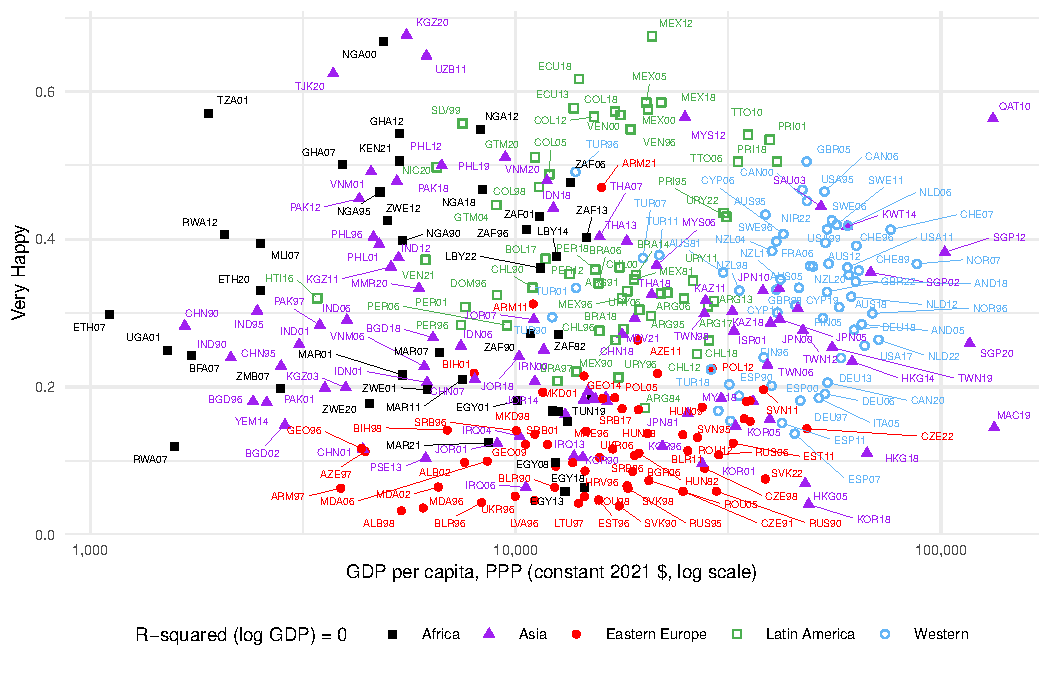
\includegraphics[width=.9\textwidth]{../figures/main/wvs_very_happy_vs_gdp_ppp.pdf}
\end{figure}

\begin{figure}[htbp]
    \centering
    \caption{Mean ladder vs.\ GDP per capita (PPP), Gallup, last observation per country}\label{fig:gallup_gdp}
    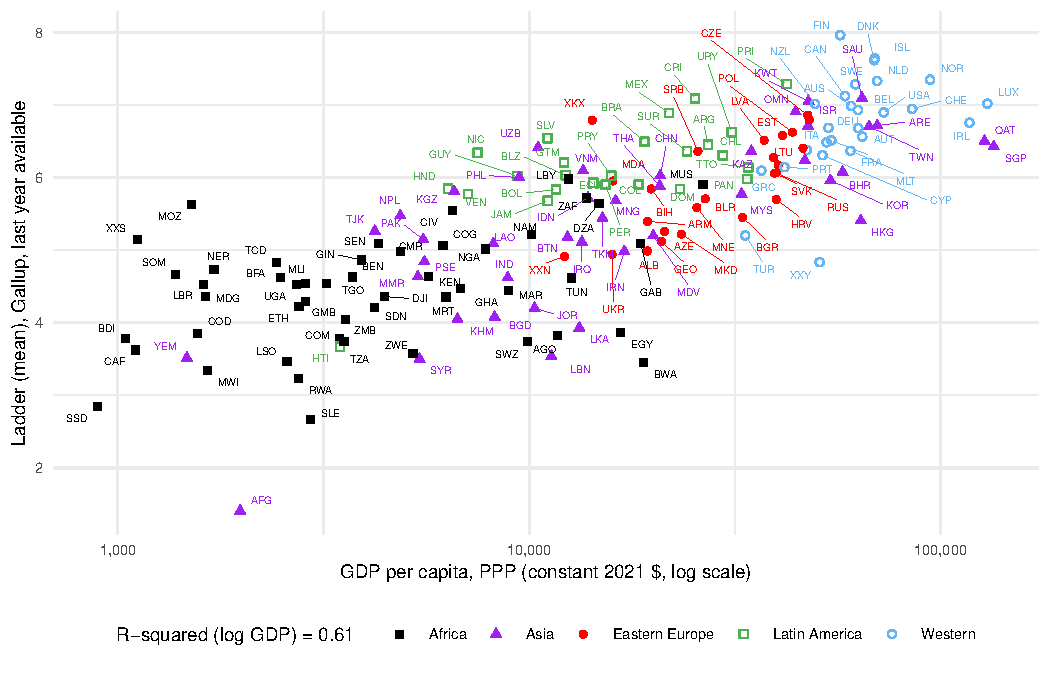
\includegraphics[width=.9\textwidth]{../figures/main/gallup_ladder_mean_vs_gdp_ppp.pdf}
\end{figure}
